%%
%% Automatically generated file from DocOnce source
%% (https://github.com/hplgit/doconce/)
%%

% #define PREAMBLE

% #ifdef PREAMBLE
%-------------------- begin preamble ----------------------

\documentclass[%
oneside,                 % oneside: electronic viewing, twoside: printing
final,                   % draft: marks overfull hboxes, figures with paths
10pt]{article}

\listfiles               %  print all files needed to compile this document

\usepackage{relsize,makeidx,color,setspace,amsmath,amsfonts,amssymb}
\usepackage[table]{xcolor}
\usepackage{bm,ltablex,microtype}

\usepackage[pdftex]{graphicx}

% Packages for typesetting blocks of computer code
\usepackage{fancyvrb,framed,moreverb}

% Define colors
\definecolor{orange}{cmyk}{0,0.4,0.8,0.2}
\definecolor{tucorange}{rgb}{1.0,0.64,0}
\definecolor{darkorange}{rgb}{.71,0.21,0.01}
\definecolor{darkgreen}{rgb}{.12,.54,.11}
\definecolor{myteal}{rgb}{.26, .44, .56}
\definecolor{gray}{gray}{0.45}
\definecolor{mediumgray}{gray}{.8}
\definecolor{lightgray}{gray}{.95}
\definecolor{brown}{rgb}{0.54,0.27,0.07}
\definecolor{purple}{rgb}{0.5,0.0,0.5}
\definecolor{darkgray}{gray}{0.25}
\definecolor{darkblue}{rgb}{0,0.08,0.45}
\definecolor{darkblue2}{rgb}{0,0,0.8}
\definecolor{lightred}{rgb}{1.0,0.39,0.28}
\definecolor{lightgreen}{rgb}{0.48,0.99,0.0}
\definecolor{lightblue}{rgb}{0.53,0.81,0.92}
\definecolor{lightblue2}{rgb}{0.3,0.3,1.0}
\definecolor{lightpurple}{rgb}{0.87,0.63,0.87}
\definecolor{lightcyan}{rgb}{0.5,1.0,0.83}

\colorlet{comment_green}{green!50!black}
\colorlet{string_red}{red!60!black}
\colorlet{keyword_pink}{magenta!70!black}
\colorlet{indendifier_green}{green!70!white}

% Backgrounds for code
\definecolor{cbg_gray}{rgb}{.95, .95, .95}
\definecolor{bar_gray}{rgb}{.92, .92, .92}

\definecolor{cbg_yellowgray}{rgb}{.95, .95, .85}
\definecolor{bar_yellowgray}{rgb}{.95, .95, .65}

\colorlet{cbg_yellow2}{yellow!10}
\colorlet{bar_yellow2}{yellow!20}

\definecolor{cbg_yellow1}{rgb}{.98, .98, 0.8}
\definecolor{bar_yellow1}{rgb}{.98, .98, 0.4}

\definecolor{cbg_red1}{rgb}{1, 0.85, 0.85}
\definecolor{bar_red1}{rgb}{1, 0.75, 0.85}

\definecolor{cbg_blue1}{rgb}{0.87843, 0.95686, 1.0}
\definecolor{bar_blue1}{rgb}{0.7,     0.95686, 1}

%\setlength{\fboxsep}{-1.5mm}  % adjust cod_vpad/pro_vpad background box

%% Background for code blocks (parameter is color name)

%% pro/cod_vpad: gives some vertical padding before and after the text
%% (but has more simplistic code than _cod/pro_tight+cod/pro).
%% pro/cod_vpad can be used to enclose Verbatim or lst begin/end for code.
%% pro/cod calls _pro/cod_tight and has very little vertical padding,
%% used to enclose Verbatim and other begin/end for code.
%% (pro/cod is what the ptex2tex program could produce with the
%% Blue/BlueBar definitions in .ptex2tex.cfg.)

\newenvironment{cod_vpad}[1]{
   \def\FrameCommand{\colorbox{#1}}
   \MakeFramed{\FrameRestore}}
   {\endMakeFramed}

\newenvironment{_cod_tight}[1]{
   \def\FrameCommand{\colorbox{#1}}
   \FrameRule0.6pt\MakeFramed {\FrameRestore}\vskip3mm}
   {\vskip0mm\endMakeFramed}

\newenvironment{cod}[1]{
\bgroup\rmfamily
\fboxsep=0mm\relax
\begin{_cod_tight}{#1}
\list{}{\parsep=-2mm\parskip=0mm\topsep=0pt\leftmargin=2mm
\rightmargin=2\leftmargin\leftmargin=4pt\relax}
\item\relax}
{\endlist\end{_cod_tight}\egroup}

%% Background for complete program blocks (parameter 1 is color name
%% for background, parameter 2 is color for left bar)
\newenvironment{pro_vpad}[2]{
   \def\FrameCommand{\color{#2}\vrule width 1mm\normalcolor\colorbox{#1}}
   \MakeFramed{\FrameRestore}}
   {\endMakeFramed}

\newenvironment{_pro_tight}[2]{
   \def\FrameCommand{\color{#2}\vrule width 1mm\normalcolor\colorbox{#1}}
   \FrameRule0.6pt\MakeFramed {\advance\hsize-2mm\FrameRestore}\vskip3mm}
   {\vskip0mm\endMakeFramed}

\newenvironment{pro}[2]{
\bgroup\rmfamily
\fboxsep=0mm\relax
\begin{_pro_tight}{#1}{#2}
\list{}{\parsep=-2mm\parskip=0mm\topsep=0pt\leftmargin=2mm
\rightmargin=2\leftmargin\leftmargin=4pt\relax}
\item\relax}
{\endlist\end{_pro_tight}\egroup}

\usepackage{minted}
\usemintedstyle{default}

\usepackage[T1]{fontenc}
%\usepackage[latin1]{inputenc}
\usepackage{ucs}
\usepackage[utf8x]{inputenc}

\usepackage{lmodern}         % Latin Modern fonts derived from Computer Modern

% Hyperlinks in PDF:
\definecolor{linkcolor}{rgb}{0,0,0.4}
\usepackage{hyperref}
\hypersetup{
    breaklinks=true,
    colorlinks=true,
    linkcolor=linkcolor,
    urlcolor=linkcolor,
    citecolor=black,
    filecolor=black,
    %filecolor=blue,
    pdfmenubar=true,
    pdftoolbar=true,
    bookmarksdepth=3   % Uncomment (and tweak) for PDF bookmarks with more levels than the TOC
    }
%\hyperbaseurl{}   % hyperlinks are relative to this root

\setcounter{tocdepth}{2}  % levels in table of contents

% Tricks for having figures close to where they are defined:
% 1. define less restrictive rules for where to put figures
\setcounter{topnumber}{2}
\setcounter{bottomnumber}{2}
\setcounter{totalnumber}{4}
\renewcommand{\topfraction}{0.95}
\renewcommand{\bottomfraction}{0.95}
\renewcommand{\textfraction}{0}
\renewcommand{\floatpagefraction}{0.75}
% floatpagefraction must always be less than topfraction!
% 2. ensure all figures are flushed before next section
\usepackage[section]{placeins}
% 3. enable begin{figure}[H] (often leads to ugly pagebreaks)
%\usepackage{float}\restylefloat{figure}

\usepackage{framed,wrapfig}

% --- begin definitions of admonition environments ---

% Admonition style "grayicon" has colored background, no frame, and an icon
% Admon "notice"
\definecolor{grayicon_notice_background}{rgb}{0.91,0.91,0.91}
% \fboxsep sets the space between the text and the box
\newenvironment{noticeshaded}
{\def\FrameCommand{\fboxsep=3mm\colorbox{grayicon_notice_background}}
 \MakeFramed {\advance\hsize-\width \FrameRestore}}{\endMakeFramed}

\newenvironment{notice_grayiconadmon}[1][Note]{
\begin{noticeshaded}
\noindent
\begin{wrapfigure}{l}{0.07\textwidth}
\vspace{-13pt}

\includegraphics[width=0.07\textwidth]{latex_figs/small_gray_notice}
\end{wrapfigure} \textbf{#1}\par
\nobreak\noindent\ignorespaces
}
{
\end{noticeshaded}
}

% Admonition style "grayicon" has colored background, no frame, and an icon
% Admon "summary"
\definecolor{grayicon_summary_background}{rgb}{0.91,0.91,0.91}
% \fboxsep sets the space between the text and the box
\newenvironment{summaryshaded}
{\def\FrameCommand{\fboxsep=3mm\colorbox{grayicon_summary_background}}
 \MakeFramed {\advance\hsize-\width \FrameRestore}}{\endMakeFramed}

\newenvironment{summary_grayiconadmon}[1][Résumé]{
\begin{summaryshaded}
\noindent
\begin{wrapfigure}{l}{0.07\textwidth}
\vspace{-13pt}
\includegraphics[width=0.07\textwidth]{latex_figs/small_gray_summary}
\end{wrapfigure} \textbf{#1}\par
\nobreak\noindent\ignorespaces
}
{
\end{summaryshaded}
}

% Admonition style "grayicon" has colored background, no frame, and an icon
% Admon "warning"
\definecolor{grayicon_warning_background}{rgb}{0.91,0.91,0.91}
% \fboxsep sets the space between the text and the box
\newenvironment{warningshaded}
{\def\FrameCommand{\fboxsep=3mm\colorbox{grayicon_warning_background}}
 \MakeFramed {\advance\hsize-\width \FrameRestore}}{\endMakeFramed}

\newenvironment{warning_grayiconadmon}[1][Avertissement]{
\begin{warningshaded}
\noindent
\begin{wrapfigure}{l}{0.07\textwidth}
\vspace{-13pt}
\includegraphics[width=0.07\textwidth]{latex_figs/small_gray_warning}
\end{wrapfigure} \textbf{#1}\par
\nobreak\noindent\ignorespaces
}
{
\end{warningshaded}
}

% Admonition style "grayicon" has colored background, no frame, and an icon
% Admon "question"
\definecolor{grayicon_question_background}{rgb}{0.91,0.91,0.91}
% \fboxsep sets the space between the text and the box
\newenvironment{questionshaded}
{\def\FrameCommand{\fboxsep=3mm\colorbox{grayicon_question_background}}
 \MakeFramed {\advance\hsize-\width \FrameRestore}}{\endMakeFramed}

\newenvironment{question_grayiconadmon}[1][Question]{
\begin{questionshaded}
\noindent
\begin{wrapfigure}{l}{0.07\textwidth}
\vspace{-13pt}
\includegraphics[width=0.07\textwidth]{latex_figs/small_gray_question2}
\end{wrapfigure} \textbf{#1}\par
\nobreak\noindent\ignorespaces
}
{
\end{questionshaded}
}

% Admonition style "grayicon" has colored background, no frame, and an icon
% Admon "block"
\definecolor{grayicon_block_background}{rgb}{0.91,0.91,0.91}
% \fboxsep sets the space between the text and the box
\newenvironment{blockshaded}
{\def\FrameCommand{\fboxsep=3mm\colorbox{grayicon_block_background}}
 \MakeFramed {\advance\hsize-\width \FrameRestore}}{\endMakeFramed}

\newenvironment{block_grayiconadmon}[1][Block]{
\begin{blockshaded}
\noindent
 \textbf{#1}\par
\nobreak\noindent\ignorespaces
}
{
\end{blockshaded}
}

% --- end of definitions of admonition environments ---

% prevent orhpans and widows
\clubpenalty = 10000
\widowpenalty = 10000

% --- end of standard preamble for documents ---


% insert custom LaTeX commands...

\raggedbottom
\makeindex
\usepackage[totoc]{idxlayout}   % for index in the toc
\usepackage[nottoc]{tocbibind}  % for references/bibliography in the toc

%-------------------- end preamble ----------------------

\begin{document}

% matching end for #ifdef PREAMBLE
% #endif

\newcommand{\exercisesection}[1]{\subsection*{#1}}


% ------------------- main content ----------------------



% ----------------- title -------------------------

\thispagestyle{empty}

\begin{center}
{\LARGE\bf
\begin{spacing}{1.25}
Chapitre 2 : Programmation Orientée Objet
\end{spacing}
}
\end{center}

% ----------------- author(s) -------------------------

\begin{center}
{\bf Ahmed Ammar}
\end{center}

    \begin{center}
% List of all institutions:
\centerline{{\small Institut Préparatoire aux Études Scientifiques et Techniques, Université de Carthage.}}
\end{center}
    
% ----------------- end author(s) -------------------------


% --- begin date ---
\begin{center}
Nov 7, 2020
\end{center}
% --- end date ---

\vspace{1cm}


\tableofcontents


\vspace{1cm} % after toc




% !split
\section{Introduction}
La Programmation Orientée Objet (POO) est une discipline de programmation dans laquelle le programmeur établit :
\begin{itemize}
\item non seulement les structures de données,

\item mais aussi les opérations qui peuvent leurs être appliquées.
\end{itemize}

\noindent
Ainsi,
\begin{itemize}
\item la structure de données devient un \textbf{objet} qui inclut
\begin{itemize}

 \item Données, appelées \textbf{attributs}

 \item Opérations, appelées \textbf{méthodes}

\end{itemize}

\noindent
\item Le programmeur peut définir des \textbf{relations} entre les objets
\end{itemize}

\noindent
% !split
\section{Classe et Objet}
\subsection{Définitions}
Une \textbf{classe} est équivalente à un nouveau type de données. On connaît déjà par exemple les classes \texttt{list} ou \texttt{str} et les nombreuses méthodes permettant de les manipuler, par exemple :
\begin{itemize}
\item \texttt{[3, 5, 1].sort()}

\item \texttt{casse.upper()}
\end{itemize}

\noindent
Un \textbf{objet} ou une \textbf{instance} est un exemplaire particulier d'une classe. Par exemple \texttt{[3, 5, 1]} est une instance de la classe \texttt{list} et \texttt{casse} est une instance de la classe \texttt{str}.

Les objets ont généralement deux sortes d'attributs : les données nommées simplement \textbf{attributs} et les fonctions applicables appelées \textbf{méthodes}.

Par exemple un objet de la classe \texttt{complex} possède :
\begin{itemize}
\item deux attributs : \texttt{imag} et \texttt{real} ;

\item plusieurs méthodes, comme \texttt{conjugate()}, \texttt{abs()}...
\end{itemize}

\noindent
La plupart des classes encapsulent à la fois les données et les méthodes applicables aux objets. Par exemple un objet \texttt{str} contient une chaîne de caractères Unicode (les données) et de nombreuses méthodes.

On peut définir un \emph{objet} comme une \emph{capsule} contenant des \textbf{attributs} et des \textbf{méthodes}.

\subsection{Création de classe en Python}
Une nouvelle classe est définie par le mot-clé \texttt{class}.

\textbf{Syntaxe de la création :}

\begin{cod}{cbg_gray}\begin{minted}[fontsize=\fontsize{9pt}{9pt},linenos=false,mathescape,baselinestretch=1.0,fontfamily=tt,xleftmargin=2mm]{python}
class NomDeLaClasse:
  # Définition des attributs de la classe
  nom_attr = valeur # attribut de valeur commune pour toutes les instances
  ...
  # Définition des attributs d'objet (chaque instance a sa propre valeur)
  def __init__(self, parametres): # le constructeur de l'objet
    self.nomattr1= v1
    self.nomattr2= v2
    ...

  # Définition des méthodes
  def nom_methode(self, autres_parametres):
    # Corps de la méthode
\end{minted}
\end{cod}
\noindent


Une classe permet de définir (déclarer) l'ensemble attributs et méthodes relatives à une catégorie d'objets.
\begin{itemize}
\item \textbf{Attributs de classe :} Un attribut de classe est défini au niveau de la classe et sa valeur est partagée par tous les objets instanciés de cette classe. L'accès à l'attribut est donné par : \Verb!NomDeLaClasse.nom_attribut!

\item \textbf{Attributs d'objets :} Un attribut d'objet est défini au niveau de la méthode constructeur. La valeur d'un attribut d'objet est propre à chaque objet. L'accès à l'attribut est donné par : \Verb!nom_Objet.nom_attribut!

\item \textbf{Le constructeur d'objet :} Le constructeur est une méthode particulière appelée lors de la création d'un nouvel objet permettant d'initialiser ses attributs. Le constructeur se définit dans une classe comme une fonction avec deux particularités~:
\begin{itemize}

  \item le nom de la méthode doit être \Verb!__init__! ;

  \item la méthode doit accepter au moins un paramètre de nom \texttt{self} qui apparaît en premier.

\end{itemize}

\noindent
\item \textbf{Le paramètre self :} Le paramètre \texttt{self} représente en fait l'objet cible, c'est-à-dire que c'est une variable qui référence l'objet en cours de création et permettant d'accéder à ses attributs et fonctionnalités.

\item \textbf{Les méthodes :} Une méthode est une fonction qui agit principalement sur une instance de la classe. Elle doit accepter au moins le paramètre \texttt{self} figurant en première position. L'appel d'une méthode se fait par : \Verb!nom_Objet.nom_méthode(autres paramètres)!
\end{itemize}

\noindent
\subsection{Exemple : Une classe pour comptes bancaires}

Le concept de compte bancaire dans un programme est un bon candidat pour un cours. Le compte comporte certaines données, généralement le nom du titulaire du compte, le numéro de compte et le solde courant. Trois choses que l'on peut faire avec un compte, c'est retirer de l'argent, mettre de l'argent sur le compte et imprimer les données du compte. Ces actions sont modélisées par des méthodes. Avec une classe, nous pouvons regrouper les données et les actions dans un nouveau type de données de sorte qu'un compte corresponde à une variable d'un programme.

Elle est créée ainsi :

\begin{pro}{cbg_gray}{bar_gray}\begin{minted}[fontsize=\fontsize{9pt}{9pt},linenos=false,mathescape,baselinestretch=1.0,fontfamily=tt,xleftmargin=2mm]{python}
# Création de la classe CompteBancaire
class CompteBancaire:
    nomBanque = 'BIAT'	#Attributs de classe
    def __init__(self, nom, num_compte, montant_initial):
	# Attributs d'objet
        self.nom = nom
        self.no = num_compte
        self.sold = montant_initial

    # Méthodes
    def depot(self, montant):
        self.sold += montant
        
    def retrait(self, montant):
        if self.sold >= montant:
            self.sold -= montant
        else:
            raise Exception('retrait impossible')
    def decharge(self):
        s = "{}, {}, solde : {}".format(self.nom, self.no, self.sold)
        print(s)
\end{minted}
\end{pro}
\noindent

La classe \texttt{CompteBancaire} définie par:
\begin{itemize}
\item \textbf{Les attributs:}
\begin{itemize}

 \item Attributs de classe : \texttt{nomBanque} (nom de la banque);

 \item Attributs d'objet : \texttt{no} (numéro du compte), \texttt{nom} (nom du propriétaire) et \texttt{sold} (solde).

\end{itemize}

\noindent
\item \textbf{Les méthodes :} \texttt{depot}, \texttt{decharge} et \texttt{retrait}.
\end{itemize}

\noindent
\begin{figure}[!ht]  % 
  \centerline{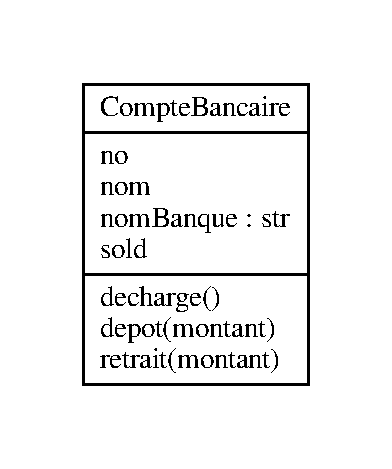
\includegraphics[width=0.5\linewidth]{scripts/classes_CompteBancaire.pdf}}
  \caption{
  Diagramme de classe \texttt{CompteBancaire}.
  }
\end{figure}
%\clearpage % flush figures 


\subsection{Création d'objets en Python}
La création d'une \textbf{instance} (objet) d'une classe donnée se fait par un appel au nom de la classe avec les paramètres effectifs du constructeur, selon la syntaxe suivante :
\begin{cod}{cbg_gray}\begin{minted}[fontsize=\fontsize{9pt}{9pt},linenos=false,mathescape,baselinestretch=1.0,fontfamily=tt,xleftmargin=2mm]{python}
>>> nom_obj = NomClasse(paramètres effectifs du constructeur)
\end{minted}
\end{cod}
\noindent

Voici un test simple de la façon dont la classe \texttt{CompteBancaire} peut être utilisée :
\begin{cod}{cbg_gray}\begin{minted}[fontsize=\fontsize{9pt}{9pt},linenos=false,mathescape,baselinestretch=1.0,fontfamily=tt,xleftmargin=2mm]{python}
>>> c1 = CompteBancaire('Mohamed Ahmed', '19371554951', 20000)
>>> c2 = CompteBancaire('Ali Tounsi',  '19371564761', 10000)
>>> c1.depot(1000)
>>> c1.retrait(4000)
>>> c2.retrait(8750)
>>> c1.retrait(1250)
>>> print("le solde de c1 : ", c1.sold)
le solde de c1 :  15750
>>> c1.decharge()
Mohamed Ahmed, 19371554951, solde : 15750
\end{minted}
\end{cod}
\noindent

\subsection{Constructeur}

Les constructeurs sont généralement utilisés pour \textbf{instancier un objet}. La tâche des constructeurs consiste à initialiser (attribuer des valeurs) aux attributs de la classe lorsqu'un objet de la classe est créé.

En Python, la méthode \Verb!__init__()! est appelée le constructeur et est toujours appelée. quand un objet est créé.

\textbf{Types de constructeurs :}

\begin{itemize}
\item \textbf{Constructeur par défaut} : le constructeur par défaut est un constructeur simple qui n’accepte aucun argument. Sa définition n’a qu’un seul argument qui soit une référence à l’instance en cours de construction.

\item \textbf{Constructeur paramétré} : Le constructeur paramétré prend son premier argument en tant que référence à l'instance en cours de construction, appelée self, et le reste des arguments est fourni par le programmeur.
\end{itemize}

\noindent
En python, on ne peut définir qu'un seul constructeur :

\begin{cod}{cbg_gray}\begin{minted}[fontsize=\fontsize{9pt}{9pt},linenos=false,mathescape,baselinestretch=1.0,fontfamily=tt,xleftmargin=2mm]{python}
class Personne:
    nom=''
    prenom=''

    # constructeur de la classe
    def __init__(self, nom, prenom):
        self.nom=nom
        self.prenom=prenom
\end{minted}
\end{cod}
\noindent

\subsection{Destructeur}
Les destructeurs sont appelés lorsqu'un objet est détruit. En Python, les destructeurs ne sont pas aussi nécessaires que en d'autres langages de programmation, car Python dispose d'un \textbf{ramasse-miettes} qui gère automatiquement la gestion de la mémoire.

La méthode \Verb!__del __()! est une méthode appelée \textbf{destructeur} en Python. Il est appelé lorsque toutes les références à l’objet ont été supprimées, c’est-à-dire lorsqu’un objet est nettoyé.

\textbf{Exemple 1 : Classe Tableau :}

Voici un exemple simple de destructeur :
\begin{cod}{cbg_gray}\begin{minted}[fontsize=\fontsize{9pt}{9pt},linenos=false,mathescape,baselinestretch=1.0,fontfamily=tt,xleftmargin=2mm]{python}
class Tableau:
    donnee=[]
    # constructeur de la classe
    def __init__(self):
        #initialiser le tableau avec 100 éléments
        self.donnee=[0]*100

    def __del__(self):
        print("je suis le destructeur")
        # vider le tableau
        self.donnee.clear()
\end{minted}
\end{cod}
\noindent
En utilisant le mot-clé \texttt{del}, nous avons supprimé toutes les références de l’objet \texttt{tab}. Le destructeur est donc invoqué automatiquement.
\begin{cod}{cbg_gray}\begin{minted}[fontsize=\fontsize{9pt}{9pt},linenos=false,mathescape,baselinestretch=1.0,fontfamily=tt,xleftmargin=2mm]{python}
>>> tab = Tableau()
>>> del tab
je suis le destructeur
\end{minted}
\end{cod}
\noindent


\begin{notice_grayiconadmon}[Note]
Le destructeur est appeler à la fin du programme ou lorsque toutes les références à l'objet ont été supprimées. C'est-à-dire que le nombre de références devient zéro, et non lorsque l'objet est sorti de la portée.
\end{notice_grayiconadmon} % title: Note



\textbf{Exemple 2 : Classe Personne :}

Cet exemple donne une explication de la note.

\begin{pro}{cbg_gray}{bar_gray}\begin{minted}[fontsize=\fontsize{9pt}{9pt},linenos=false,mathescape,baselinestretch=1.0,fontfamily=tt,xleftmargin=2mm]{python}
class Personne:
 
    # constructeur de la classe
    def __init__(self, nom, prenom):      
        self.nom = nom
        self.prenom = prenom
 
    def __del__(self): 
        print("je suis le destructeur")
\end{minted}
\end{pro}
\noindent

\begin{cod}{cbg_gray}\begin{minted}[fontsize=\fontsize{9pt}{9pt},linenos=false,mathescape,baselinestretch=1.0,fontfamily=tt,xleftmargin=2mm]{python}
def creation():
    print("creation de l'objet")
    p = Personne('TOUNSI','Mohamed')
    print('fin de la création')
    return p

print("Début du programme")
p1=creation()
print("Je suis {} {}, je suis un objet d'ID : {}".format(p1.nom, p1.prenom, id(p1)))
print("fin du programme")
del p1
\end{minted}
\end{cod}
\noindent
Notez que le destructeur est appelé après l'affichage de \emph{"Fin du programme..."}

\section{Méthodes spéciales et surcharge des opérateurs}
Certaines méthodes de classe ont des noms qui commencent et se terminent par un double trait de soulignement. Ces méthodes permettent une syntaxe spéciale dans le programme et sont appelées \textbf{méthodes spéciales}. Le constructeur \Verb!__init__()! en est un exemple. Cette méthode est automatiquement appelée lorsqu'une instance est créée, mais nous n'avons pas besoin d'écrire explicitement \Verb!__init__()!. D'autres méthodes spéciales permettent d'effectuer des opérations arithmétiques avec des instances, de comparer des instances avec \texttt{>}, \texttt{>=}, \Verb?!=?, etc., d'appeler des instances comme nous appelons les fonctions ordinaires, et de tester si une instance évalue à Vrai ou Faux, pour mentionner certaines possibilités.

La \textbf{surcharge} permet à un opérateur de \textbf{posséder un sens différent} suivant le \textbf{type} de ses opérandes.

Par exemple, l'opérateur \texttt{+} permet :
\begin{cod}{cbg_gray}\begin{minted}[fontsize=\fontsize{9pt}{9pt},linenos=false,mathescape,baselinestretch=1.0,fontfamily=tt,xleftmargin=2mm]{python}
x = 7 + 9 # addition entière
s = 'ab' + 'cd' # concaténation
\end{minted}
\end{cod}
\noindent
Python possède des méthodes de surcharge pour :
\begin{itemize}
\item tous les types (\Verb!__call__!, \Verb!__str__! ...) ;

\item les nombres (\Verb!__add__!, \Verb!__div__! ...) ;

\item les séquences (\Verb!__len__!, \Verb!__iter__! ...).
\end{itemize}

\noindent
\subsection{Surcharge de l'appel fonctionnel}
La méthode \Verb!__call__! permet aux programmeurs Python d'écrire des classes dont les instances se comportent comme des fonctions et peuvent être appelées comme une fonction. Lorsque l'instance est appelée comme une fonction ; si cette méthode est définie, \texttt{objet(arg1, arg2, ...)} est une abréviation de \Verb!objet.__call__(arg1, arg2, ...)!.

\textbf{Exemple :}

\begin{cod}{cbg_gray}\begin{minted}[fontsize=\fontsize{9pt}{9pt},linenos=false,mathescape,baselinestretch=1.0,fontfamily=tt,xleftmargin=2mm]{python}
class Produit:
	def __init__(self):
		print("Création de l'instance")

	# Définir la méthode __call__.
	def __call__(self, a, b):
		print(a * b)

# Création de l'instance
ans = Produit()

# La méthode __call__ sera appelée
ans(10, 20)
\end{minted}
\end{cod}
\noindent

\subsection{Représentation formelle d'un objet}

Pour afficher les informations relatives à un objet, en utilisant le nom de l'objet (représentation sur le shell) ou en utilisant la commande \texttt{print()} , il faut surcharger la méthode spéciale \Verb!__repr__! :
\begin{cod}{cbg_gray}\begin{minted}[fontsize=\fontsize{9pt}{9pt},linenos=false,mathescape,baselinestretch=1.0,fontfamily=tt,xleftmargin=2mm]{python}
def __repr__(self):
  return #la chaine qu'on veut afficher
\end{minted}
\end{cod}
\noindent

\textbf{Exemple :}

\begin{cod}{cbg_gray}\begin{minted}[fontsize=\fontsize{9pt}{9pt},linenos=false,mathescape,baselinestretch=1.0,fontfamily=tt,xleftmargin=2mm]{python}
class point:
    def __init__(self,a,b):
        self.x=a
        self.y=b
    def __repr__(self):
        return (str((self.x , self.y)))
\end{minted}
\end{cod}
\noindent

\begin{cod}{cbg_gray}\begin{minted}[fontsize=\fontsize{9pt}{9pt},linenos=false,mathescape,baselinestretch=1.0,fontfamily=tt,xleftmargin=2mm]{python}
>>> p=point(2,3)
>>> p # l'exécution de l'évaluation de p fait appel à __repr__
(2,3)
>>> print(p) # l'exécution de print fait appel à la méthode __repr__
(2,3)
\end{minted}
\end{cod}
\noindent

\subsection{Représentation informelle d'un objet}

Pour donner une représentation textuelle informelle à un objet, il suffit de surcharger la méthode spéciale \Verb!__str__! :
\begin{cod}{cbg_gray}\begin{minted}[fontsize=\fontsize{9pt}{9pt},linenos=false,mathescape,baselinestretch=1.0,fontfamily=tt,xleftmargin=2mm]{python}
def __str__(self):
  return #la chaine qu'on veut afficher
\end{minted}
\end{cod}
\noindent

\textbf{Exemple 1 :}

\begin{cod}{cbg_gray}\begin{minted}[fontsize=\fontsize{9pt}{9pt},linenos=false,mathescape,baselinestretch=1.0,fontfamily=tt,xleftmargin=2mm]{python}
class point:
    def __init__(self,a,b):
        self.x=a
        self.y=b
    def __str__(self):
        return 'point' + str((self.x , self.y))
\end{minted}
\end{cod}
\noindent

\begin{cod}{cbg_gray}\begin{minted}[fontsize=\fontsize{9pt}{9pt},linenos=false,mathescape,baselinestretch=1.0,fontfamily=tt,xleftmargin=2mm]{python}
>>> p = point(2,3)
>>> p #sans redéfinir __repr__ l'exécution renvoie la référence de l'objet
<__main__.point object at 0x033DAB10>
>>> print(p) # l'exécution de print fait appel à la méthode __str__
point(2,3)
\end{minted}
\end{cod}
\noindent

\textbf{Exemple 2 :}

\begin{cod}{cbg_gray}\begin{minted}[fontsize=\fontsize{9pt}{9pt},linenos=false,mathescape,baselinestretch=1.0,fontfamily=tt,xleftmargin=2mm]{python}
class point:
    def __init__(self,a,b):
        self.x=a
        self.y=b
    def __repr__(self):
        return str((self.x , self.y))
    def __str__(self):
        return 'point' + str((self.x , self.y))
\end{minted}
\end{cod}
\noindent

\begin{cod}{cbg_gray}\begin{minted}[fontsize=\fontsize{9pt}{9pt},linenos=false,mathescape,baselinestretch=1.0,fontfamily=tt,xleftmargin=2mm]{python}
>>> p = point(2,3)
>>> p # l'exécution de l'évaluation de p fait appel à __repr__
(2,3)
>>> print(p) # l'exécution de print fait appel à la méthode __str__
point(2,3)
\end{minted}
\end{cod}
\noindent

\subsection{Surcharge des opérateurs}
La surcharge d'opérateurs permet la redéfinition et l'utilisation des opérateurs en fonction de la classe. Par exemple, l'utilisation de l'opérateur \texttt{+} pour additionner deux objets de même type.

Python associe à chaque opérateur une méthode spéciale qu'on peut surcharger, on cite dans la suite quelques
exemples :
\begin{itemize}
\item Exemples des méthodes spéciales permettant la surcharge des opérateurs arithmétiques :
\begin{itemize}

 \item opérateurs unaires :
\begin{itemize}

  \item \texttt{+} : \Verb!__pos__(self)!

  \item \texttt{-} : \Verb!__neg__(self)!

\end{itemize}

\noindent
 \item opérateurs binaires :
\begin{itemize}

  \item \texttt{+} : \Verb!__add__(self,other)!

  \item \texttt{*} : \Verb!__mul__(self, other)!

  \item \texttt{-} : \Verb!__sub__(self,other)!

  \item ...

\end{itemize}

\noindent
\end{itemize}

\noindent
\item Exemples des méthodes spéciales permettant la surcharge des opérateurs de comparaison :
\begin{itemize}

 \item \texttt{==} : \Verb!__eq__(self,other)!

 \item \Verb?!=? : \Verb!__ne__(self, other)!

 \item \texttt{>} : \Verb!__gt__(self,other)!

 \item ...

\end{itemize}

\noindent
\item Exemples des méthodes spéciales permettant la surcharge des opérateurs d'indexation :
\begin{itemize}

 \item \texttt{objet[i]} : \Verb!__getitem__(self,indice)!

 \item \texttt{objet[i] = v} : \Verb!__setitem__(self,indice,valeur)!
\end{itemize}

\noindent
\end{itemize}

\noindent
\subsection{Exemple : Classe pour les vecteurs dans le plan}
Cette partie explique comment implémenter des vecteurs bidimensionnels en Python de telle sorte que ces vecteurs agissent comme des objets que nous pouvons ajouter, soustraire, former des produits internes avec, et faire d'autres opérations mathématiques.

Les vecteurs dans le plan sont décrits par une paire de nombres réels, $(a,b)$. Il existe des règles mathématiques pour ajouter et soustraire des vecteurs, multiplier deux vecteurs (le produit intérieur ou point ou scalaire), la longueur d'un vecteur, et la multiplication par un scalaire :
\begin{align}
(a,b) + (c,d) &= (a+c, b+d),\\
(a,b) - (c,d) &= (a-c, b-d),\\
(a,b)\cdot(c,d) &= ac + bd,\\
||(a,b)|| &= \sqrt{(a,b)\cdot(a,b)}.
\end{align}
De plus, deux vecteurs $(a,b)$ et $(c,d)$ sont égaux si $a=c$ et $b=d$.
\paragraph{Implémentation.}
Nous pouvons créer une classe pour les vecteurs de plan où les opérations mathématiques ci-dessus sont mises en œuvre par des méthodes spéciales. La classe doit contenir deux attributs de données, un pour chaque composante du vecteur, appelés \texttt{x} et \texttt{y} ci-dessous. Nous incluons des méthodes spéciales pour l'addition, la soustraction, le produit scalaire (multiplication), la valeur absolue (longueur), la comparaison de deux vecteurs (\texttt{==} et \Verb?!=?), ainsi qu'une méthode pour imprimer un vecteur.

\begin{pro}{cbg_gray}{bar_gray}\begin{minted}[fontsize=\fontsize{9pt}{9pt},linenos=false,mathescape,baselinestretch=1.0,fontfamily=tt,xleftmargin=2mm]{python}
import math as m
class Vec2D(object):
    def __init__(self, x, y):
        self.x = x
        self.y = y

    def __add__(self, other):
        return Vec2D(self.x + other.x, self.y + other.y)

    def __sub__(self, other):
        return Vec2D(self.x - other.x, self.y - other.y)

    def __mul__(self, other):
        return self.x*other.x + self.y*other.y

    def __abs__(self):
        return m.sqrt(self.x**2 + self.y**2)

    def __eq__(self, other):
        return self.x == other.x and self.y == other.y

    def __str__(self):
        return '({:g}, {:g})'.format(self.x, self.y)

    def __ne__(self, other):
        return not self.__eq__(other)  # réutiliser __eq__
\end{minted}
\end{pro}
\noindent
Les méthodes \Verb!__add__!, \Verb!__sub__!, \Verb!__mul__!, \Verb!__abs__!, et \Verb!__eq__! devraient être assez simples à comprendre d'après les définitions mathématiques précédentes de ces opérations. La dernière méthode mérite un commentaire : ici, nous réutilisons simplement l'opérateur d'égalité \Verb!__eq__!, mais nous le faisons précéder d'un non. Nous aurions également pu mettre en oeuvre cette méthode comme :
\begin{cod}{cbg_gray}\begin{minted}[fontsize=\fontsize{9pt}{9pt},linenos=false,mathescape,baselinestretch=1.0,fontfamily=tt,xleftmargin=2mm]{python}
def __ne__(self, autre):
        return self.x != other.x or self.y != other.y
\end{minted}
\end{cod}
\noindent

\paragraph{Utilisation.}
Prenons quelques objets Vec2D :
\begin{cod}{cbg_gray}\begin{minted}[fontsize=\fontsize{9pt}{9pt},linenos=false,mathescape,baselinestretch=1.0,fontfamily=tt,xleftmargin=2mm]{python}
>>> u = Vec2D(0,1)
>>> v = Vec2D(1,0)
>>> w = Vec2D(1,1)
>>> a = u + v
>>> print(a)
(1, 1)
>>> a == w
True
>>> a = u - v
>>> print(a)
(-1, 1)
>>> a = u*v
>>> print(a)
0
>>> print(abs(u))
1.0
>>> u == v
False
>>> u != v
True
\end{minted}
\end{cod}
\noindent
Lorsque vous lisez cette présentation interactive, vous devez vérifier que le calcul est mathématiquement correct, que le type d'objet résultant d'un calcul est correct et que chaque calcul est effectué dans le programme. Ce dernier point est étudié en suivant le déroulement du programme à travers les méthodes de classe. À titre d'exemple, considérons l'expression \Verb?u != v?. Il s'agit d'une expression booléenne qui est \texttt{True} puisque u et v sont des vecteurs différents. Le type d'objet résultant doit être \texttt{bool}, avec des valeurs \texttt{True} ou \texttt{False}.

\section{Héritage et polymorphisme}
Un avantage décisif de la POO est qu'une classe Python peut toujours être spécialisée en une classe \textbf{fille} qui \textbf{hérite} alors de tous les attributs (données et méthodes) de sa \textbf{super classe} (classe mère). Comme tous les attributs peuvent être redéfinis, une méthode de la classe fille et de la classe mère peut posséder le même nom, mais effectuer des traitements différents (\textbf{surcharge}) et l'objet s'adaptera dynamiquement, dès l'instanciation. En proposant d'utiliser un même nom de méthode pour plusieurs types d'objets différents, le \textbf{polymorphisme} permet une programmation beaucoup plus générique. Le développeur n'a pas à savoir, lorsqu'il programme une méthode, le type précis de l'objet sur lequel la méthode va s'appliquer. Il lui suffit de savoir que cet objet implémentera la méthode.

L'héritage se fait ainsi selon la syntaxe suivante :
\begin{cod}{cbg_gray}\begin{minted}[fontsize=\fontsize{9pt}{9pt},linenos=false,mathescape,baselinestretch=1.0,fontfamily=tt,xleftmargin=2mm]{python}
class nom_sous_classe(nom_classe_mère):
  #définir les attributs et les méthodes de la sous_classe
\end{minted}
\end{cod}
\noindent


\begin{notice_grayiconadmon}[Note]
L'héritage est le mécanisme qui permet de se servir d'une classe préexistante pour en créer une nouvelle qui possédera des fonctionnalités supplémentaires ou différentes.

Le \emph{polymorphisme} par \emph{dérivation} est la faculté pour deux méthodes (ou plus) portant le même nom, mais appartenant à des classes héritées distinctes d'effectuer un travail différent. Cette propriété est acquise par la technique de la \textbf{surcharge}.
\end{notice_grayiconadmon} % title: Note



\subsection{Exemple d'héritage et de polymorphisme}
Dans l'exemple suivant, la classe \texttt{QuadrupedeDebout} hérite de la classe mère \texttt{Quadrupede}, et la méthode \texttt{piedsAuContactDuSol()} est polymorphe :

\begin{pro}{cbg_gray}{bar_gray}\begin{minted}[fontsize=\fontsize{9pt}{9pt},linenos=false,mathescape,baselinestretch=1.0,fontfamily=tt,xleftmargin=2mm]{python}
class Quadrupede:
    def piedsAuContactDuSol(self):
        return 4

class QuadrupedeDebout(Quadrupede):
    def piedsAuContactDuSol(self):
        return 2
\end{minted}
\end{pro}
\noindent


\begin{figure}[!ht]  % 
  \centerline{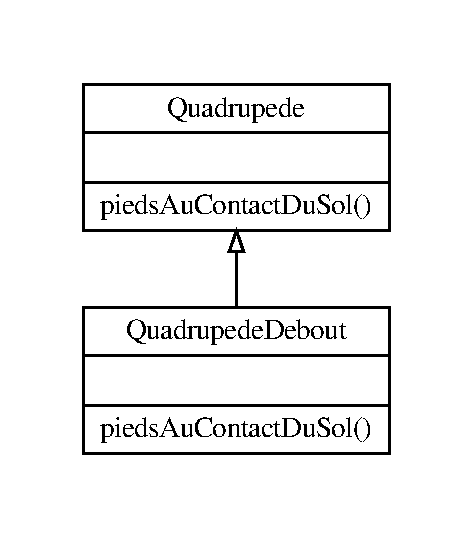
\includegraphics[width=0.5\linewidth]{scripts/classes_Quadrupede.pdf}}
  \caption{
  Diagramme de classe \texttt{Quadrupede} et sa fille \texttt{QuadrupedeDebout}.
  }
\end{figure}
%\clearpage % flush figures 


Voici un test simple de la façon dont ces classes \texttt{Quadrupede} et \texttt{QuadrupedeDebout} peuvent être utilisées :
\begin{cod}{cbg_gray}\begin{minted}[fontsize=\fontsize{9pt}{9pt},linenos=false,mathescape,baselinestretch=1.0,fontfamily=tt,xleftmargin=2mm]{python}
>>> chat = Quadrupede()
>>> chat.piedsAuContactDuSol()
4
>>> homme = QuadrupedeDebout()
>>> homme.piedsAuContactDuSol()
2
\end{minted}
\end{cod}
\noindent
\subsection{Exemple d'héritage et de dérivation}

La dérivation décrit la création de sous-classes par spécialisation. Elle repose sur la relation « est-un ».

On utilise dans ce cas le mécanisme de l'héritage.

L'implémentation Python utilisée est généralement l'appel à l'initialisateur de la classe parente dans l'initialisateur de la classe dérivée (utilisation de la fonction \texttt{super()}).

Dans l'exemple suivant, un \textbf{Carre} « est-un » \textbf{Rectangle} particulier pour lequel on appelle l'initialisateur de la classe mère avec les paramètres \texttt{longueur=cote} et \texttt{largeur=cote} :

\begin{pro}{cbg_gray}{bar_gray}\begin{minted}[fontsize=\fontsize{9pt}{9pt},linenos=false,mathescape,baselinestretch=1.0,fontfamily=tt,xleftmargin=2mm]{python}
class Rectangle:
    def __init__(self, longueur=30, largeur=15):
        self.L, self.l = longueur, largeur
        self.nom = "rectangle"
    def __str__(self):
        return "nom : {}".format(self.nom)

class Carre(Rectangle): # héritage simple
    """
    Sous-classe spécialisée de la super-classe Rectangle.
    """
    def __init__(self, cote=20):
        # appel au constructeur de la super-classe de Carre :
        super().__init__(cote, cote)
        self.nom = "carré" # surcharge d'attribut
\end{minted}
\end{pro}
\noindent

L'utilisation est comme suivant :

\begin{cod}{cbg_gray}\begin{minted}[fontsize=\fontsize{9pt}{9pt},linenos=false,mathescape,baselinestretch=1.0,fontfamily=tt,xleftmargin=2mm]{python}
>>> r = Rectangle()
>>> c = Carre()
>>> print(r)
nom : rectangle
>>> print(c)
nom : carré
\end{minted}
\end{cod}
\noindent

\section{Application : Création des classes Pile et File}
\subsection{La classe Pile}
\paragraph{Définition d'une pile.}
On rappelle qu'une pile est une structure de données qui suit le principe d'une pile d'assiettes, "*le dernier arrivé est le premier sorti*", on parle du mode \textbf{LIFO} (Last In First Out). L'insertion ou la suppression d'un élément ne peut se faire qu'à une seule extrémité, appelée sommet de la pile.

Une pile est définie par les opérations suivantes :
\begin{itemize}
\item \textbf{Empiler} : permet l'ajout d'un élément au sommet de la pile ;

\item \textbf{Dépiler} : permet la suppression de l'élément au sommet de la pile si elle n'est pas vide ;

\item \textbf{Vérifier} si une pile est vide ou non.
\end{itemize}

\noindent
\paragraph{Implémentation d'une classe Pile.}
La classe Pile est définie par :
\begin{itemize}
\item L'attribut :
\begin{itemize}

 \item liste : initialisé par une liste vide

\end{itemize}

\noindent
\item Les méthodes :
\begin{itemize}

 \item \texttt{empiler} : permet l'ajout d'un élément donné à la fin de l'attribut \texttt{liste};

 \item \texttt{depiler} : permet de supprimer et retourner le dernier élément de l'attribut \texttt{liste} s'il existe;

 \item \Verb!est_vide! : permet de vérifier si l'attribut \texttt{liste} est vide ou non.
\end{itemize}

\noindent
\end{itemize}

\noindent
\begin{cod}{cbg_gray}\begin{minted}[fontsize=\fontsize{9pt}{9pt},linenos=false,mathescape,baselinestretch=1.0,fontfamily=tt,xleftmargin=2mm]{python}
class Pile:
    def __init__(self) :
        self.liste=[]
    def empiler (self, v) :
        self.liste.append(v)
    def depiler(self) :
        if self.est_vide() == False:
            return self.liste.pop()
    def est_vide(self) :
        return self.liste == []
    def __repr__(self):
        return (str(self.liste))
\end{minted}
\end{cod}
\noindent

\subsection{La classe File}
\paragraph{Définition d'une File.}
On rappelle qu'une file est une structure de données qui suit le principe d'une file d'attente, "le premier arrivé est le premier sorti", on parle du mode \textbf{FIFO} (First In First Out).

Une file est définie par les opérations suivantes :
\begin{itemize}
\item \textbf{enfiler} : permet l'ajout d'un élément la fin de la file ;

\item \textbf{défiler} : permet la suppression de l'élément au début de la file si elle n'est pas vide;

\item \textbf{vérifier} si une file est vide ou non.
\end{itemize}

\noindent
\paragraph{Implémentation d'une classe File.}
La classe File est définie par :
\begin{itemize}
\item L'attribut :
\begin{itemize}

 \item liste : initialisé par une liste vide

\end{itemize}

\noindent
\item Les méthodes :
\begin{itemize}

 \item \texttt{enfiler} : permet l'ajout d'un élément donné à la fin de l'attribut \texttt{liste};

 \item \texttt{defiler} : permet de supprimer et retourner le premier élément de l’attribut \texttt{liste} s’il existe;

 \item \Verb!est_vide! : permet de vérifier si l'attribut \texttt{liste} est vide ou non.
\end{itemize}

\noindent
\end{itemize}

\noindent
\begin{cod}{cbg_gray}\begin{minted}[fontsize=\fontsize{9pt}{9pt},linenos=false,mathescape,baselinestretch=1.0,fontfamily=tt,xleftmargin=2mm]{python}
class File:
    def __init__(self) :
        self.liste=[]
    def enfiler (self, v) :
        self.liste.append(v)
    def defiler(self) :
        if self.est_vide() == False:
              return self.liste.pop(0)
    def est_vide(self) :
        return self.liste == []
    def __repr__(self):
        return (str(self.liste))
\end{minted}
\end{cod}
\noindent

\subsection{Exemple d'inversion d'une pile}
Il s'agit d’écrire une fonction \texttt{Inverser(p)} qui permet d’inverser une pile \texttt{p} :
\begin{itemize}
\item avec utilisation d'une file intermédiaire ;

\item sans utilisation d'une file intermédiaire.
\end{itemize}

\noindent
\begin{cod}{cbg_gray}\begin{minted}[fontsize=\fontsize{9pt}{9pt},linenos=false,mathescape,baselinestretch=1.0,fontfamily=tt,xleftmargin=2mm]{python}
# en utilisant une file intermédiaire
def Inverser(p):
    f1 = File()
    while not p.est_vide():
        f1.enfiler(p.depiler())
    while not f1.est_vide():
        p.empiler(f1.defiler())
\end{minted}
\end{cod}
\noindent

\begin{cod}{cbg_gray}\begin{minted}[fontsize=\fontsize{9pt}{9pt},linenos=false,mathescape,baselinestretch=1.0,fontfamily=tt,xleftmargin=2mm]{python}
>>> p = Pile()
>>> p.empiler(2)
>>> p.empiler(6)
>>> p.empiler(8)
>>> p
[2, 6, 8]
>>> Inverser(p)
>>> p
[8, 6, 2]
\end{minted}
\end{cod}
\noindent


\begin{cod}{cbg_gray}\begin{minted}[fontsize=\fontsize{9pt}{9pt},linenos=false,mathescape,baselinestretch=1.0,fontfamily=tt,xleftmargin=2mm]{python}
# sans utiliser une file intermédiaire
def Inverser(p):
    p1 = Pile()
    p2 = Pile()
    while not p.est_vide():
        p1.empiler(p.depiler())
    while not p1.est_vide():
        p2.empiler(p1.depiler())
    while not p2.est_vide():
        p.empiler(p2.depiler())
\end{minted}
\end{cod}
\noindent
\begin{cod}{cbg_gray}\begin{minted}[fontsize=\fontsize{9pt}{9pt},linenos=false,mathescape,baselinestretch=1.0,fontfamily=tt,xleftmargin=2mm]{python}
>>> print(p)
[8, 6, 2]
>>> Inverser(p)
>>> print(p)
[2, 6, 8]
\end{minted}
\end{cod}
\noindent

% ------------------- end of main content ---------------

% #ifdef PREAMBLE
\end{document}
% #endif

